\documentclass[a4paper,11pt]{kth-mag}
\usepackage[T1]{fontenc}
\usepackage{textcomp}
\usepackage{lmodern}
\usepackage[latin1]{inputenc}
\usepackage[swedish,english]{babel}
\usepackage{modifications}
\usepackage{graphicx} % Required to insert images
\usepackage{hyperref}
\usepackage[nameinlink, capitalise]{cleveref}
\usepackage{longtable}
\newcolumntype{P}[1]{>{\centering\arraybackslash}p{#1}}

% För formateringen av en rapport/artikel finns ofta färdiga mallar. Publicerar man t.ex. en artikel på en konferens eller i en tidskrift finns mallar/anvisningar som beskriver vilka typsnitt, storlekar, radavstånd, marginaler paragrafnumrering etc. som skall användas.
% Ofta beskrivs också hur lång texten får vara i antal ord och antal sidor.
% För den här uppgiften skall texten ligga mellan 7 och 12 sidor oräknat försättsblad, Abstract, sammanfattning, referenslista och bilagor.

% Den här rapportmallen beskriver vad man kan förvänta sig finna i en teknisk rapport som baseras på någon form av undersökning/utredning. De rubriker/stycken som är beskrivna är de som återfinns i de allra flesta rapporter. För längre rapporter delar man ofta upp rapporten i flera stycken med egna rubriker. T.ex. kanske man beskriver flera olika experiment och experimentuppställningar.

% I rapporten kan och bör du återanvända delar av det du skrivit i din projektplanering.

% Försättssida: Titeln skall vara deskriptiv/informativ. Sätts i Arial 14 punkter fet stil (KTH titel)

% Försättssida: Här anger man namn på alla författare, titlar och kontaktinformation
\title{Priority Queues Experiment}
\subtitle{November 20, 2016}
\foreigntitle{Lorem ipsum dolor sit amet, sed diam nonummy nibh eui mod tincidunt ut laoreet dol}
\author{Wong, Sai Man\\ Tigerstr\"{o}m, Gabriel}
\date{November 2016}
\blurb{}
\trita{}
\begin{document}
\frontmatter
\pagestyle{empty}
\removepagenumbers
\maketitle
\selectlanguage{english}

% Ny sida- startar på högersida: I examensarbetsrapporter på KTH skall det finnas sammanfattning på både svenska och engelska (Abstract). Rubriken sätts i Arial 12 punkter fet stil ( KTH rubrik), brödtexten som  Times New Roman 10 punkter (KTH Brödtext)
\begin{abstract}
This is a skeleton for KTH theses. More documentation
regarding the KTH thesis class file can be found in
the package documentation.

Lorem ipsum dolor sit amet, consectetuer adipiscing elit. Mauris
purus. Fusce tempor. Nulla facilisi. Sed at turpis. Phasellus eu
ipsum. Nam porttitor laoreet nulla. Phasellus massa massa, auctor
rutrum, vehicula ut, porttitor a, massa. Pellentesque fringilla. Duis
nibh risus, venenatis ac, tempor sed, vestibulum at, tellus. Class
aptent taciti sociosqu ad litora torquent per conubia nostra, per
inceptos hymenaeos.
\end{abstract}
\clearpage

% Ny sida, startar på högersida. Sammanfattning och Abstract skall innehålla samma text men på olika språk. Sammanfattningen skall översiktligt beskriva vad rapporten innehåller och de viktigaste resultaten. Den hålls normalt ganska kortfattad (1/4-1/2 A4 sida text. De skrivs på separata sidor.
\begin{foreignabstract}{swedish}
Denna fil ger ett avhandlingsskelett.
Mer information om \LaTeX-mallen finns i
dokumentationen till paketet.

Lorem ipsum dolor sit amet, consectetuer adipiscing elit. Mauris
purus. Fusce tempor. Nulla facilisi. Sed at turpis. Phasellus eu
ipsum. Nam porttitor laoreet nulla. Phasellus massa massa, auctor
rutrum, vehicula ut, porttitor a, massa. Pellentesque fringilla. Duis
nibh risus, venenatis ac, tempor sed, vestibulum at, tellus. Class
aptent taciti sociosqu ad litora torquent per conubia nostra, per
inceptos hymenaeos.
\end{foreignabstract}
\clearpage

% Om man har ett bra verktyg som man skriver sin rapport i och man använder väldefinierade paragraf/stilmallar så kan innehållsförteckningen oftast automatgenereras
\tableofcontents*
\mainmatter
\pagestyle{newchap}

% ///////////////////////////////////
% ///////////////////////////////////
%           Introduction
% ///////////////////////////////////
% ///////////////////////////////////
% Huvudrubriker sätts i Arial 12 punkter fet stil autonumrerad (KTH nRubrik 1).
% Här introducerar man problemomådet. Här skall finnas en bakgrund till projektet, de problem man adresserar/undersöker och syftet med arbetet.De olika underkapitlen/styckena till introduktionen  förtydligar det du skriver här. Här förväntar man sig hitta ett antal noga utvalda hög-kvalitativa referenser.
\chapter{Introduction}
% Underrubriker (första nivån) sätts i Arial 12 punkter fet stil autonumrerad (KTH  nRubrik 2). (Har man ytterligare undernivåer sätter man rubrikerna för nästa nivå  med (KTH nRubrik 3)) Man försöker ofta begäränsa sig till tre nivåer på rubriker och man har i princip aldrig fler än 4 nivåer på rubriker.

% I stycket om bakgrund (som ibland kallas ”Related work” på engelska) förväntar man sig hitta en gedigen bakgrundsbeskrivning till problemområdet i stort och till det specifika problem som studeras i rapporten. Den skall innehålla/baseras på en litteraturstudie. Det behöver väl knappast påpekas att den bör innehålla utvalda, högkvalitativa referenser.
\section{Background}
The data type \emph{queue} is represented as a \emph{first in first out} (FIFO) data structure \cite{deshpande2004c}.
That is, the first element enqueued in the queue is the first one that becomes dequeued.
Another usage this data type is a priority queue.
For example, an implementation of a process and thread scheduler in an operating system.
In a priority queue, each element is enqueued based on their priority values in either decreasing or increasing order.
A priority queue can thus be implemented with a data structure called \emph{linked list}, or a \emph{doubly linked list} that was used in this project.
It is a model to store data in dynamic lists during runtime.

Another data structure that can be used to represent a priority queue is the \emph{splay tree} \cite{sleator1985self}.


% Här beskriver du problemområdet och problemet i detalj. Beskriv också varför det är värdefullt att undersöka problemet. Försök formulera din problemställning så klart och koncist som möjligt – gärna i en mening!
\section{Problem Statement}

% Om detta är en studie där syftet är att undersöka en hypotes (alla projekt är inte hypotesprövande) så beskriver du/formulerar du hypotesen här. Lämpligt är också att beskriva hur/varför/på vilka grunder du formulerat hypotesen. Är det inte ett hypotesprövande projekt så tar du bort rubriken.
\section{Hypothesis}

% Beskriv varför projektet genomförs.
\section{Purpose}
The purpose of this experiment was to gain real life experience on how to carry out an experiment methodically.
That is, a well-planned experiment of high quality.
It was thus emphasized to research different scientific methods to design, implement and test the implementation.

% Beskriv de förväntade resultat- och effektmålen av undersökningen. Beskriv alla mål du satt upp även om de inte nåddes!
\newpage
\section{Goal}
\label{sec:goal}
The goals were to evaluate two different data structures for a priority queue.
These may be summerized as follows:
\begin{itemize}
    \item Doubly linked list - Insert new elements from the front or rear
        \begin{itemize}
            \item Front: if the new element's priority value is \textbf{higher} than the mean of the first and last element
            \item Rear: if the new element's priority value is \textbf{lower} than the mean of the first and last element
        \end{itemize}
    \item Splay Tree \cite{sleator1985self}
        \begin{itemize}
            \item A self adjusting binary search tree invented by Daniel Sleator och Robert Tarjan (WHERE IS THIS EXPLAINED)
        \end{itemize}
\end{itemize}
% A model for the requirement overview was set up and presented in \cref{app:A} before any code was written, which is the MoSCoW model to design a plan as described in \cref{sec:srem}.
The MoSCoW model, described in \cref{sec:srem}, was implemented in this experiment.
This model was used to set up the plan and requirements, which are presented in \cref{app:A}.

% Samhallsnytta, etik och hallbar utveckling
% Beskriv vem och på vilket sätt man kan ha nytta av utredningen. Beskriv etiska och hållbar utvecklingsrelaterade frågor kopplade till utredningen.
\section{Social Benefit, Ethics and Sustainable Development}

% Om man har eller behöver införa avgränsningar av studien (som inte är uppenbara) så kan man beskriva dem i ett speciellt stycke.
\section{Delimitation}
The goal of this experiment was achieved by a sufficient amount of data.
But also with such reliability analytical conclusions were drawn from.
% 3.3.4 Delimitation ?!?!?
% The goal of the experiment has been achieved when there is a dataset sufficient and reliable enough to draw analytical conclusions from. There is no magic number of how many iterations or combinations to try, but if the experiment only has to be executed once the goal is achieved. There is no real upper limit on the precision of the experiment but given the nature of this experiment it can be quite coarse. As long as there are distinctions between the iterations and combinations the experiment is finished. As seen in Section A: Table 2 Row 6-9, the experiments requirements (i.e. what need to be tested) are listed. When these four requirements are fulfilled the experiment is finished.

% I större, mer omfattande rapporter med flera stycken lägger man ibland till en översikt Disposition (Overview) som beskrivar vad läsaren kommer att hitta i de olika styckena. Syftet är att hjälpa läsaren få en översikt över rapporten så han/hon kan hitta snabbt i den.
\section{Outline}

% ///////////////////////////////////
% ///////////////////////////////////
%       Method and Methodology
% ///////////////////////////////////
% ///////////////////////////////////

% I metoelen beskriver du den vetenskapliga metod du baserat ditt projekt på.
%
% Vilka relevanta metoder finns? Vilka har du övervägt att använda? Varför valde du den/de metoder du använt?
%  Beskriv kort den metod du använt och hur du applicerat den - dvs. vilken data du samlar in, hur du gör det och varför. Beskriv också tillförlitligheten hos data du samlar in. Går experimenten att upprepa? Finns etiska eller HU aspekter på ditt arbete.
\chapter{Method and Methodology}

\section{Inductive and Deductive Method}
An inductive method can be approached to observe a system \cite{robertdraft}.
At first it is important to gather and analyze information.
And later on form a hypothesis, and eventually, conclusions can be drawn from these observations.
Also, the inductive method is sometimes called a bottom-up design.
It is because you begin to observe information, detect patterns and formulate hypotheses.
Finally and hopefully, conclusions and theories can be reached \cite{web:induction}.

A deductive method can be seen as the opposite of an inductive method.
That is, a top-down approach rather than bottom-up.
Firstly, a deductive method begins with theories.
These theories are then narrowed down to hypotheses and observations.
Tests are set up and executed to conceivably confirm that the theories are valid.
It is common in, for example, mathematics.
In mathematics, logical and theoretical reasoning are first carried out.
And then hopefully, logical conclusions can be drawn from the reasoning.

\section{Quantitative and Qualitative Method}
A quantitative method often include tests and experiments \cite{haakansson2013portal}.
That is due to that the gathered information or data are measurable.
The experiments can then help you to either falsify or verify a hypothesis.
An example is to set up an experiment to prove the correctness of a computer system's behavioral.
A large amount of data, logic and statistics are thus required to execute such experiment and prove its validity.

In a qualitative method, the data is gathered in a smaller scale in contrary to the latter mentioned method.
This data is efficient enough to reach valid results.
For example, it is common implemented method in social sciences.
Principally to to understand people \cite{merriam2009qualitative}.
The data are often collected from interviews, observations and documentations.
It then makes up a base for further analysis and conceivably reach valid conclusions.

\section{Software Testing}
% Over around three decades, there have been four different and acknowledged methods for software testing. These have, eventually, been emerged into what is so called \emph{chess pieces}, which is considered to be the choice for successful testing \cite{bk:chesspieces}. The four approaches are as follow:
There have recently been four different and acknowledged methods for software testing called \emph{chess pieces} \cite{bk:chesspieces}.
These are considered to be the be the choice for successful testing.
The four approaches are as follow:

\begin{itemize}
    \item Static testing - test documentation, for example, requirements, design and specifications
    \item White box testing - test the internal software, for example, the source code (logic paths)
    \item Black box testing - test the external software, for example, the executable code (behavior)
    \item Performance testing - test the final software, for example, the speed of the program
\end{itemize}

\subsection{Static Testing}
The static testing includes the initial phase of software development.
That is the software's design phase.
It has been shown that 85 percent of all encountered software defects are during the design phase \cite{bk:chesspieces}.
Usually it begins, continues and ends with the documentation in the process of software development.
This is the cause for big number of software defects that \cite{bk:chesspieces} identified.
To minimize the defects the documentation must therefore be properly designed before any code can be written.
It was additionally suggested to inspect the documentation regularly during the development.
Finally as the program runs, to also present and go through the documentation.

\subsection{White Box Testing}
The developers often have access to the source code in white box texting.
It includes both the source code and executable.
Their responsibility is to understand the source code.
That is, the program specifications, standards and logic.
It is hence required that the lines in the source code are reviewed and tested in a methodical fashion.
For example, reviewed for different reasons, such as, in practice and for business purposes.
That is why white box testing can be divided into positive and negative testing respectively.

The developers in positive testing have knowledge of its internal design.
Their purpose is to prove that the code work according to the documentation.
In contrast, the developers that execute the negative testing possess knowledge of the user's perspective.
That is to find out if users can break the program by accident or on purpose.
These two approaches are shown to be most effective to find defects in white box testing.
White box testing is conclusively to test the internal design.
And also to test that the software fulfills its purpose.

\subsection{Black Box Testing}
In black box testing the developers and users only have access to the executable code.
It is often approached by a group of testers, developers and users.
The testers prepare a plan of the execution and test.
That is, both positive and negative testing as described in the last section.
Developers further possess the software's behavioral knowledge and can relate it to business purposes.
Finally, the users only have to test that the software behaves properly.
For example, from a user's business perspective.

\subsection{Performance Testing}
Performance testing is often carried out after the latter mentioned tests have been approached.
This it to make sure that the program behaves as it supposed to, statistic- and logically.
The common approach is to test the software's throughput and response time.
That is to take measurements and relate it to its execution.
To set up a test environment and identify relevant tools are thus important in performance testing.
For example, input a large amount of transaction to test the software's response time and performance.
It may also be known as load testing.
For performance testing it is hence required to be structured and log the performances to identify that the software works as intended.

\clearpage

\section{Software Development}

\subsection{Waterfall}
Waterfall method is a linear type of framework.
It is divided into sequential phases and allows phases to overlap.
This contributes to more flexibility, as shown in \cref{fig:waterfall} \cite{rep:devmethod}.
It is therefore emphasized to set up a plan, time schedules, target dates and resources needed for the implementation.
This method is suited for inexperienced project due to its linear type of framework with strict steps.
The Waterfall method ensures and facilitates the work for higher quality, more reliable and maintainable software.
Nevertheless, there is little room to work in iteration due to its strict structure.
Defects and problems are also not often discovered until the end stage of the "waterfall".
That is, when tests on the system are performed.

\begin{figure}[h!]
    \centering
    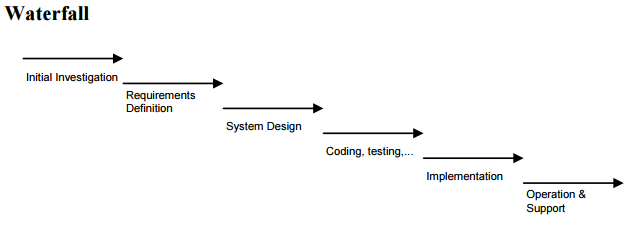
\includegraphics[scale=0.8]{waterfall.png}
    \caption{Waterfall software development method \cite{rep:devmethod}}
    \label{fig:waterfall}
\end{figure}

\subsection{Incremental with Prototyping}
The prototype method is an iterative method.
This method may also be combined with an incremental development methodology, as shown in \cref{fig:prototyping}.
As a result it becomes a combination between an iterative and a linearly approach towards software development.
This approach is considered to be more flexible than the Waterfall method.
It instead breaks down the Waterfall phases into smaller segments of the implementation.
That is that a segment must be completed before the next increment.
As you may have noticed, this is a gradual approach.
This makes it easier to identify changes.
However, the downside is that it does not take the overall system into consideration.
Instead each incremental step must be finished before the next one.

\begin{figure}[h!]
    \centering
    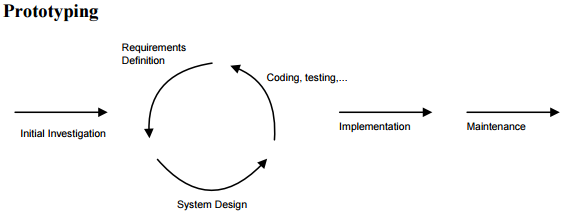
\includegraphics[scale=0.8]{prototyping.png}
    \caption{Prototyping software development method \cite{rep:devmethod}}
    \label{fig:prototyping}
\end{figure}

\section{Software Requirement Engineering Methodology}
\label{sec:srem}
A software requirement engineering model is important to set up.
Especially before the software project has begun.
The model used in this project to design specifications and requirements is presented in this section.

The requirement and specifications must be established throughout the entire project.
These are set up before the project has begun.
This is to facilitate the work within the group or project.
That is to work towards the same purpose and goal.
The model presented in \cite{eklund2011arbeta} is the MoSCoW model.
This model includes different priorities that can be set on requirements to achieve a certain purpose, as follows:

\begin{itemize}
    \item \textbf{Must} - requirements that must be fulfilled in specified time
    \item \textbf{Should} - requirements that also must be fulfilled, but at a later time
    \item \textbf{Could} - requirements that may be good to fulfill, but only if time allows and it is not critical for the project
    \item \textbf{Won't} - requirements that are not established in the project, but may be relevant to consider in the future
\end{itemize}
\clearpage
An example of how a requirement overview may be modeled is demonstrated in \cref{tab:reqoverview}.
It was designed based on the table on the course website of \emph{II1304 Engineering Skills for ICT} \cite{web:requirementoverview}.

\begin{table}
    \centering
    \caption{Requirement analysis/requirement overview from course website \cite{web:requirementoverview}}
    \label{tab:reqoverview}
    \resizebox{\textwidth}{!}{%
        \begin{tabular}{ |P{2cm}||P{2cm}|P{1.9cm}|P{5cm}|P{3cm}| }
            \hline
            \multicolumn{5}{|c|}{Specification of requirements} \\
            \hline
            Requirement number & Requirement type & Name or source &Clarified description of the requirement, followed by what should be fulfilled& Fulfilled or not fulfilled or partly fulfilled\\
            \hline
            Numbers to facilitate references to the specified requirement & Must/ Should/ Could/ Won't, followed by justification  & Descriptive name of the requirement, followed by the source of the requirement&Clarified description of the requirement. What must be fulfilled according to the requirement. If you do your own interpretations of the requirement, make sure it is clearly specified it is your own interpretation & Is the requirement fulfilled or not. It may be relevant in larger project to specify when and by whom the requirement was fulfilled by\\
            \hline
    \end{tabular}}
\end{table}

% Beskriv hur du samlar in data, material och annat underlag för din undersökning? Svara på frågor som: Hur skall undersökningen genomföras? Hur är experimentuppställningen organiserad?
\section{Data Collection}
This project applied an inductive method for data collection.
The data were collected from the implementation of the experiment.
These were then used as observations to conceivably reach valid conclusions.
This section describes the model used to execute this experiment.
And also how the experiment was organized.

The goals were identified in \cref{sec:goal}.
These goals were divided into smaller chunks with the MoSCoW model.
The two implementation were then later experimented upon.
The purpose was to generate data to analyze and draw conclusions from.

The goal of the experiment was to run iterations of the two implemented priority queues with different data set of input.
That is, the initial size, input size, stochastic distribution and other global set of variables.
The output taken from each iteration included data as run time, exit code, errors and performance.

To run only one iteration does not reveal anything significant about the implemented priority queues.
Several iterations with different inputs are thus necessary to be able to analyze the output data from the experiment.
A test framework was set up to automate these iterations.

The observations collected were numerical and in a larger scale.
It is therefore possible to apply a quantitative method on this experiment.
This approach opens up opportunities to control and guide the experiment.
That is, it is controllable such that it can give a better understanding of the theories within computer science.
For example, a deeper understanding in algorithms and data structure to implement priority queues.

\subsection{Resources}
There are requirements for resources needed to be set up to conduct an experiment and analyze the output.
To do this, the following points of data are required:
\begin{itemize}
    \item Global variables (that is, stochastic distribution of variables)
    \item Data set size of the input
    \item Running time for the simulation
    \item Does the simulation execute as predicted
\end{itemize}

With help of these points of data a correlation can be found between running time and input.
This may result in a better understanding of the algorithm experimented upon.
In addition, a correlation of global variables, fixed input size and running time can verify the algorithms correctness.
That is, the best, worst and average time complexity of the priority queues with a Doubly Linked List and the Splay Tree.

\subsection{Error and Uncertainty}
The internal sources for errors and uncertainties can be input size, stochastic distribution of inputs and the implemented data structure.
In contrast, the external sources can be CPU caching, CPU and OS scheduling or compilation optimization.
These uncertainties can have negative impact on the output.
It is thus necessary to take countermeasures to minimize the effect of skewed results.
A faulty image of the implementation can be represented if no countermeasures are taken.
One of the countermeasure can be to run the simulation several times.
As it often generates a normal distribution of values.
The extracted values can then produce a more valid mean value rather than a distorted one.

% Beskriv metoden för hur du avser analysera insamlad data/material. Beskriv också hur du planerar tolka  data..
\section{Data Analysis}
Deductive reasoning was applied in this project to analyze the data.
The analysis was based on a large quantity of observations.
These observations are then fitted into a logical reasoning.
That is, to conduct an experiment that produces results that may be verified and validated with the theory.
The reached conclusions and data need to be verified and validated, as described in the following sections.

\subsection{Verification and Validation}
To verify the experiment, one compares the result from the implementation and experiments.
The requirement specifications must also be taken into consideration.
An experiment is verified once every requirements are fulfilled.
This also includes the verification of the implementation.
There is no point to only verify the requirements related to the experiment,
if the experiment itself is also dependent on the implementation.

To validate the experiment following key points need to be accounted for \cite{haakansson2013portal}:

\begin{itemize}
    \item Validity, make sure the measurements are correct
    \item Reliability, test results show a consistency between measurements
    \item Replicability, how would someone else go about to repeat this experiment
    \item Dependability, how reliable are the drawn conclusions from the data
\end{itemize}

All these points must be accounted for in the final experiment report along with the presentation of data.
These points also play a central part in the design of the actual experiment.
This is important for the experiment due to the ability to yield the correct format of data.

% ///////////////////////////////////
% ///////////////////////////////////
%       System Description
% ///////////////////////////////////
% ///////////////////////////////////

% Ett kapitel om Systembeskrivning / Konstruktion eller i detta fall Experimentuppställning  finns inte med i alla studier men ofta i tekniska rapporter där man konstruerat ett system. Den här delen kan vara ett kapitel/stycke eller flera beroende på hur stort arbete man gjort.

% Här startar man normalt med en beskrivning av det/de system man utvecklat och /eller haft som underlag i studien.
\chapter{System Description}

% Om du utvecklat ett system (som algoritmerna för minnesallokering och testbädden) så bör du beskriva vilken/vilka metoder och verktyg du använt för systemutvecklingen. I större undersökningar/arbeten vill man gärna också se en diskussion om olika alternativ och varför man valt de man använt.
\section{Method of System Development}

% Det här är en anpassad rubrik för just den här studien. Här beskriver du (ev. med flera underrubriker) mer i detalj de algoritmer du implementerat och hur du implementerat dem.
\section{Algorithms for Priority Queue}
\subsection{Doubly Linked List}
\subsection{Splay Tree}





% Testbädd eller Experimentuppställning. Också en rubrik specifik för den här undersökningen – men också vanlig i många undersökningar där man utvärderar ett tekniskt system.
%
% Här beskriver du mer i detalj din experimentuppställning. Vilken hårdvara, OS har du kört på. Hur har du försökt minimera felkällor (sominverkan av andra användare).
% Beskriv de testfall du använt och implementerat. Argumentera för varför de är rimliga/bra.
\section{Testing}

% ///////////////////////////////////
% ///////////////////////////////////
%              Results
% ///////////////////////////////////
% ///////////////////////////////////

% Här presenterar du dina resultat och slutsatser från undersökningen. Tänk på att presentera resultaten på ett tydligt sätt och ta med tillräckligt mycket i presentationen så att alla slutsatser är tydligt välgrundade. Lyft fram det som är mest intressant och viktigt.
\chapter{Results}

% Här kan du fördjupa din diskussion och ta ett helhetsgrepp på din undersökning, metodval och resultat.
\section{Discussion}

% ///////////////////////////////////
% ///////////////////////////////////
%     Conclusions and Future Work
% ///////////////////////////////////
% ///////////////////////////////////

% Kan också kallas Diskussion eller Analys.
% Börja med att diskutera målen och syftet med undersökningen och hur väl du nått dem. Summera de viktigaste slutsatserna/upptäckterna och avsluta med att diskutera hur arbetet skulle kunna fortsättas/utvecklas (speciellt om du inte nått alla delmål)
\chapter{Conclusions and Future Work}

% I Bilagor (som inte alltid behöver finnas med) lägger man vid behov utökad information som man inte tar upp/redovisar i detalj i den ordinarie texten.
%
% För den här uppgiften är Bilagorna 1-3 sådana som man kan förvänta sig finnas med i en teknisk rapport om det specifika problem du studerat i den här uppgiften. Bilaga 4 skall innehålla de saker som efterfrågas i ID2206 för att rapporten skall kunna godkännas som labrapport i den kursen.
\appendix
\addappheadtotoc
\chapter{Requirement Overview}\label{app:A}
% ////////////////////////////////////////////////////////////////////////////////
% ////////////////////////////////////////////////////////////////////////////////
% ////////////////////////////////////////////////////////////////////////////////
% ////////////////////////////////////////////////////////////////////////////////
% //////////////////// CHANGE THIS!!! ////////////////////////////////////////////
% ////////////////////////////////////////////////////////////////////////////////
% ////////////////////////////////////////////////////////////////////////////////
% ////////////////////////////////////////////////////////////////////////////////
% ////////////////////////////////////////////////////////////////////////////////

{\footnotesize
    \begin{longtable}{ |P{2cm}||P{1.7cm}|P{2.2cm}|P{4.3cm}|P{2.3cm}| }
        \caption{Requirement overview of priority queue experiments} \label{tab:requirementoverviewexperiment}\\
        \hline
        \multicolumn{5}{|c|}{Specification of requirements for priority queue experiment} \\
        \hline
        Requirement number & Requirement type & Name or source &Clarified description of the requirement, followed by what should be fulfilled& Fulfilled or not fulfilled or partly fulfilled\\
        \hline
        1 & \textbf{Must} \newline mandatory task & Experiment plan \newline \textbf{Source:} course website & Construct a plan with relevant method, methodologies and models to carry out the experiment. \newline \textbf{Fulfilled:} write a plan for the experiment and be approved of your mentor (in our case approved by Robert R\"{o}nngren). & \textbf{Partly fulfilled} \\
        \hline
        2 & \textbf{Must} \newline mandatory task & Singly linked list (front) \newline \textbf{Source:} course website & Priority queue with an implementation of a singly linked list with insertion of new elements from the front. \newline \textbf{Fulfilled} if fully tested, i.e., its functionality in relation to the experiment model. & \textbf{Not fulfilled} \\
        \hline
        3 & \textbf{Must} \newline mandatory task & Doubly linked list (rear) \newline \textbf{Source:} course website & Priority queue with an implementation of a doubly linked list with insertion of new elements from the rear. \newline \textbf{Fulfilled} if fully tested, i.e., its functionality in relation to the experiment model & \textbf{Not fulfilled} \\
        \hline
        4 & \textbf{Must} \newline mandatory task & Doubly linked list (front/rear) \newline \textbf{Source:} course website & Priority queue with an implementation of a doubly linked list with insertion of new elements from the front or rear depending on mean of the first and last element. Front: priority value higher than mean. \newline Rear: priority value lower than mean. \newline \textbf{Fulfilled} if fully tested, i.e., its functionality in relation to the experiment model. & \textbf{Not fulfilled} \\
        \hline
        5 & \textbf{Must} \newline mandatory task & Scheduler with singly linked list (front) \newline \textbf{Source:} course website & Scheduler for managing processes or threads. \newline Priority values in the interval [0,40] where the lowest value has highest priority. \newline Each priority has a queue (FIFO property), implemented with a singly linked list with insertion from the front. \newline \textbf{Fulfilled} if fully tested, i.e., its functionality in relation to the experiment model. & \textbf{Not fulfilled} \\
        \hline
        6 & \textbf{Should} \newline mandatory task & Experiment \#1 \newline \textbf{Source:} course website & Correlate size of input with running-time for the four implementations in requirement number 2, 3, 4 and 5. \newline \textbf{Fulfilled:} when the experiments and the results has been documented. & \textbf{Not fulfilled} \\
        \hline
        7 & \textbf{Should} \newline mandatory task & Experiment \#2 \newline \textbf{Source:} authors & Correlate different stochastic distributions with running-time for the four implementations in requirement number 2, 3, 4 and 5. \newline \textbf{Fulfilled:} when the experiments and the results has been documented. & \textbf{Not fulfilled} \\
        \hline
        8 & \textbf{Could} \newline optional task & Experiment \#3 \newline \textbf{Source:} authors & Change type of data structure for implementation with requirement number 5 (scheduler) to doubly linked list. \newline \textbf{Fulfilled:} go through/perform experiment 1 and 2 (requirement number 6 and 7) again, but with doubly linked list for scheduler. Document the experiment and results in order to fulfill this requirement. & \textbf{Not fulfilled} \\
        \hline
        9 & \textbf{Could} \newline optional task & Experiment \#4 \newline \textbf{Source:} authors & Implement singly linked list. \newline \textbf{Fulfilled:} go through/perform experiment 1, 2 and eventually 3 (requirement number 6, 7 and eventually 8) again, but with circular linked list for scheduler. Document the experiment and results in order to fulfill this requirement. & \textbf{Not fulfilled} \\
        \hline
        10 & \textbf{Won't} \newline optional task & OS scheduling \newline \textbf{Source:} authors & Apply implementation for practical usage within an arbitrary operating system \newline \textbf{Fulfilled:} test the functionalities and eventually perform an arbitrary experiment & \textbf{Not fulfilled} \\
        \hline
\end{longtable}}
    \begin{figure}[ht]
        \begin{center}
            And here is a figure
            \caption{\small{Several statements describing the same resource.}}\label{RDF_4}
        \end{center}
    \end{figure}

    that we refer to here: \ref{RDF_4}

    \clearpage
    % Här listar du dina referenser. De skall täcka in alla relevanta delar  i din bakgrund, vara väl utvalda (dvs. hålla för källkritik).
    %
    % I den här rapporten använder du ISO690 numerisk variant för referenserna.
    %
    % Har man ett bra verktyg som man skriver i/hantera referenserna i så kan referenslistan automatgenereras. Det gör det också lättare att uppdatera referenslistan utan att behöva gå igenom varje referens i texten manuellt. Dessutom får man bara med källor som man refererat till minst en gång från texten.
    \bibliographystyle{IEEEtran}
    \bibliography{IEEEabrv,sources}
    \end{document}
